\documentclass{beamer}
\usetheme{Madrid}
\usepackage{lmodern}
\usepackage{hyperref}
\usepackage{apacite}
\usepackage[utf8]{inputenc}
\usepackage[spanish]{babel}

\usepackage{xcolor}
\setbeamertemplate{background}{\tikz[overlay,remember picture]\node[opacity=0.2]at (current page.center){
\includegraphics[width=13cm]{KL.png}};}
\usepackage{tikz}
\usepackage{kantlipsum}

\setbeamercolor{normal text}{fg=black}

\begin{document}
\colorlet{beamer@blendedblue}{blue!46!green}
\setbeamercolor{normal text}{fg=black}

\setbeamercolor{frametitle}{fg=white, bg=blue!46!green}
\setbeamercolor*{title}{bg=blue!46!green, fg=white}

\setbeamercolor{section in toc}{fg=black}

\author[Juan C. Correa \textcolor{white}{(\url{https://correajc.com}})]{Juan C. Correa, Ph.D.}
\title[Enseñanza basada en reproducibilidad]{Enseñanza basada en reproducibilidad}
\subtitle{Evaluación de Propiedades Psicométricas}
	%\subtitle{}
\institute[]{Fundación Universitaria Konrad Lorenz\\
	\color{blue}\Email  \href{mailto:juanc.correan@konradlorenz.edu.co}{juanc.correan@konradlorenz.edu.co}}
\pgfdeclareimage[height=0.5cm]{KL}{KL}
\logo{\pgfuseimage{KL}}
\setbeamertemplate{caption}[numbered]
\date[Bogotá, Junio-2021]{Curso en: \textbf{T}ecnologías \textbf{R}eproducibles en la \textbf{E}nseñanza de la \textbf{M}etodología y la \textbf{E}stadística}

%\subject{}
\setbeamercolor{background canvas}{bg=white}
%\setbeamertemplate{navigation symbols}{}

\begin{frame}
	\titlepage
\end{frame}

\begin{frame}
\begin{block}{Objetivo del Curso}
\vspace{0.3cm}
Comprender, a través del paquete \textbf{ShinyItemAnalysis} y algunas de sus bases de datos, los beneficios de adoptar nuevas tecnologías reproducibles para la enseñanza de contenidos metodológicos y estadísticos.
\end{block}
\end{frame}



\begin{frame}
\frametitle{Agenda} 
\tableofcontents
\end{frame}

\section{Justificación de la herramienta}
\begin{frame}{Justificación de la herramienta}
\tiny{\textcolor{blue}{\url{https://journal.r-project.org/archive/2018/RJ-2018-074/RJ-2018-074.pdf}}}
\begin{figure}
\centering
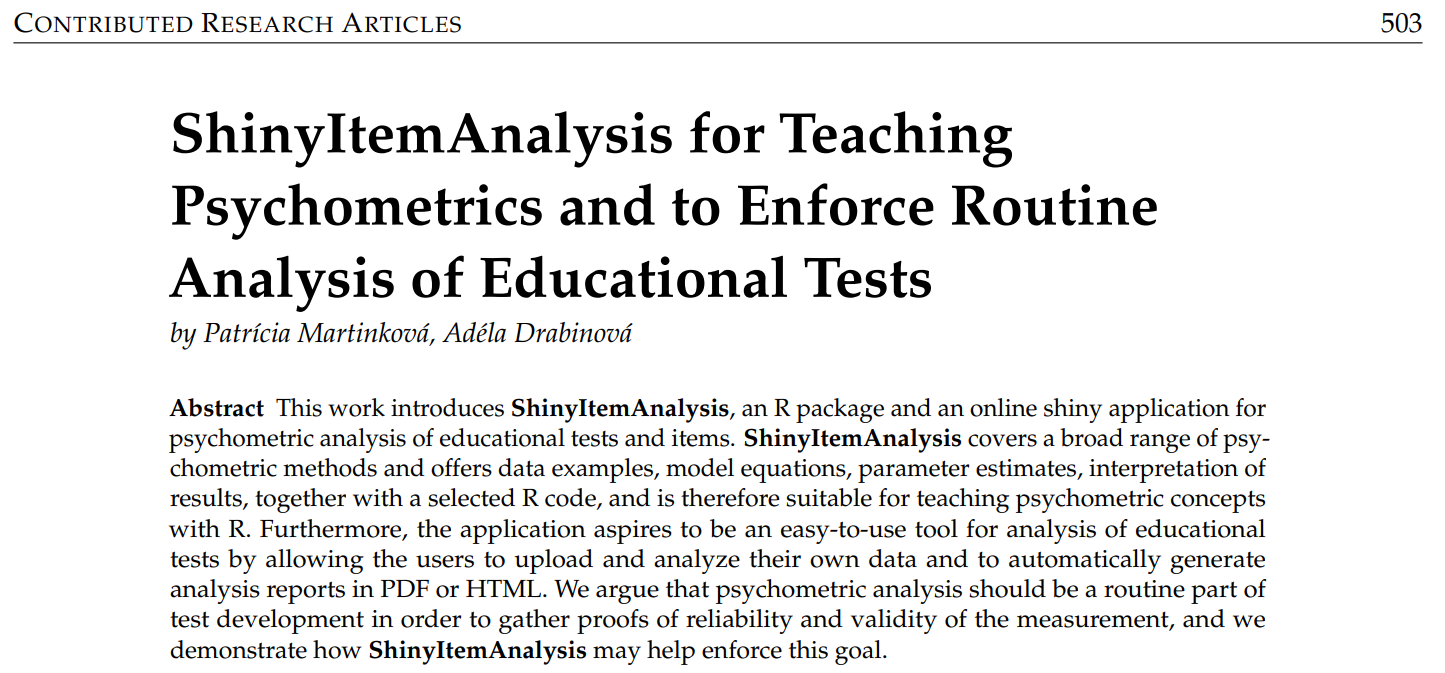
\includegraphics[width=1\textwidth]{ShinyItemAnalysis.png}
\end{figure}
\cite{Martinkova2018}
\end{frame}

\begin{frame}{Justificación de la Herramienta}
``\textit{Las evaluaciones que se utilizan para medir la capacidad o el conocimiento de los estudiantes deben producir puntajes válidos, confiables y justos. Si bien muchos paquetes de R se han desarrollado para cubrir conceptos psicométricos generales (e.g., \texttt{psych}, \texttt{ltm}) o temas psicométricos específicos (e.g., \texttt{difR}, \texttt{lavaan}), las partes interesadas en esta área a menudo no son programadores y
por lo tanto, puede resultarle difícil superar la carga inicial de un entorno basado en R. El software disponible comercialmente ofrece una alternativa, pero los altos precios y la metodología limitada pueden ser un problema.}''\\
\cite[p. 503]{Martinkova2018}
\end{frame}

\section{Requerimientos Técnicos}
\begin{frame}{Requerimientos Técnicos}
Para seguir el paso a paso de este tutorial, es necesario que usted haya instalado R y Rstudio en su computador. Acá tiene un video tutorial que le indica cómo hacerlo (\textcolor{blue}{\url{https://youtu.be/Bg2LzHmPZFY}}).
\begin{figure}
\centering

\includegraphics[width=.7\textwidth]{Chupitos.png}
\end{figure}      
\end{frame}

\section{ShinyItemAnalysis: Tutorial paso-a-paso}
\begin{frame}
\Huge
\centering
\texttt{ShinyItemAnalysis} \\
Tutorial Paso-a-Paso\\
(En Rstudio Escritorio)
\end{frame}


\begin{frame}{ShinyItemAnalysis: Paso 1}
Ingresamos a RStudio 
\begin{figure}
\centering
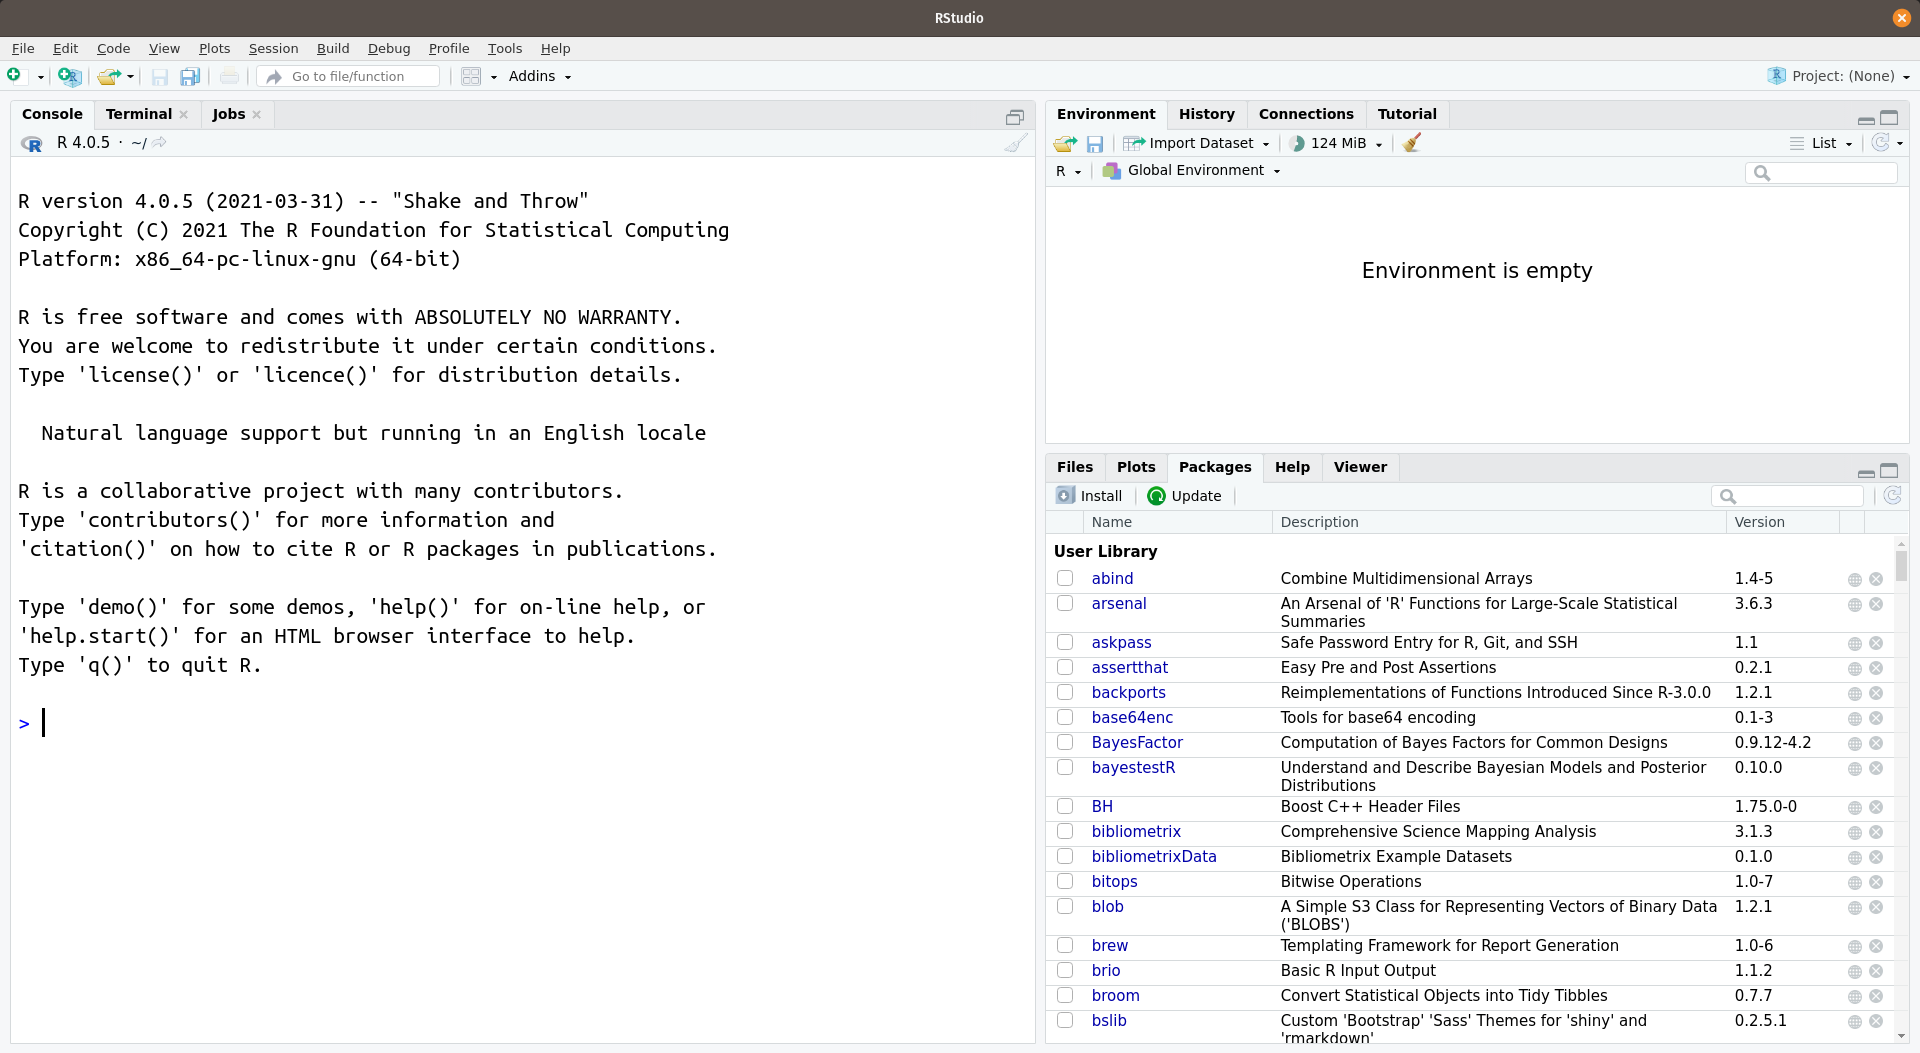
\includegraphics[width=.95\textwidth]{Apariencia.png}
\end{figure}  
\end{frame}

\begin{frame}{ShinyItemAnalysis: Paso 2}
Vamos a la pestaña Packages
\begin{figure}
\centering
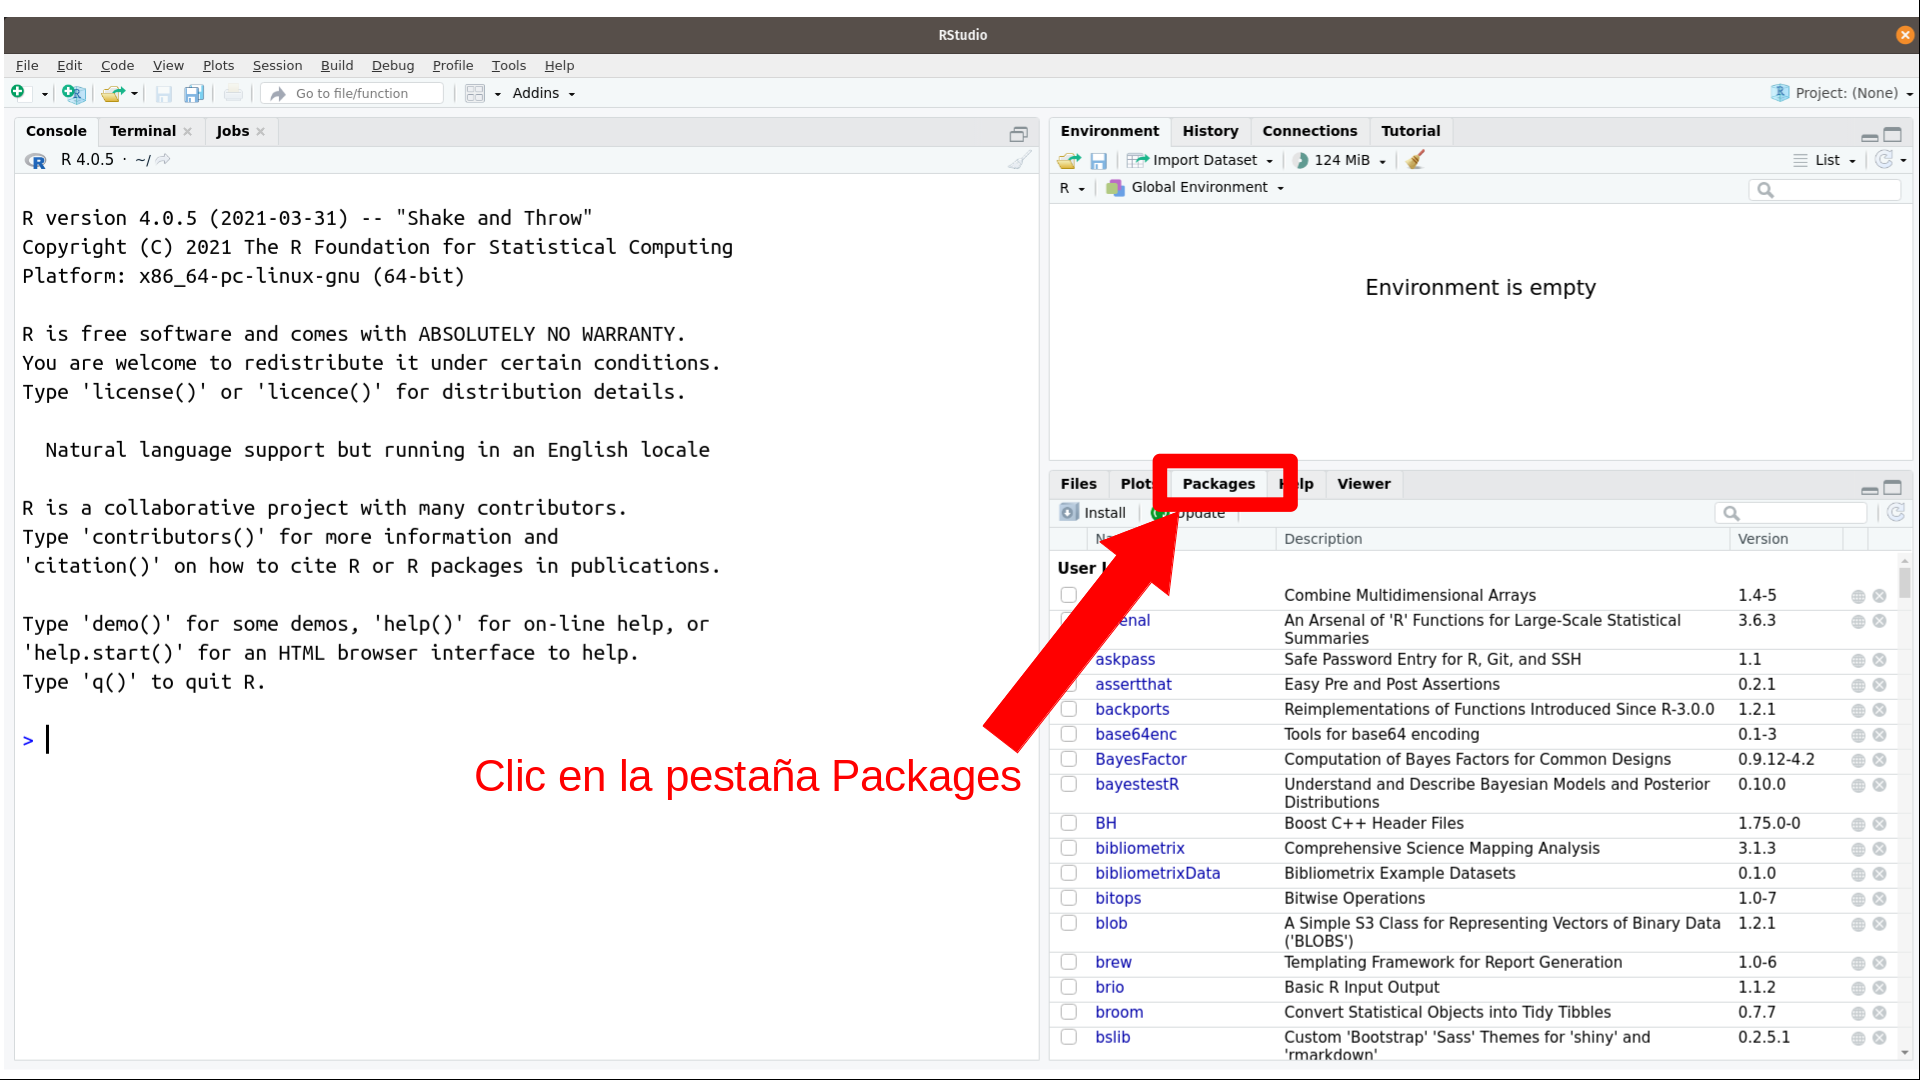
\includegraphics[width=.92\textwidth]{Paso1.png}
\end{figure}  
\end{frame}

\begin{frame}{ShinyItemAnalysis: Paso 3}
\begin{figure}
\centering
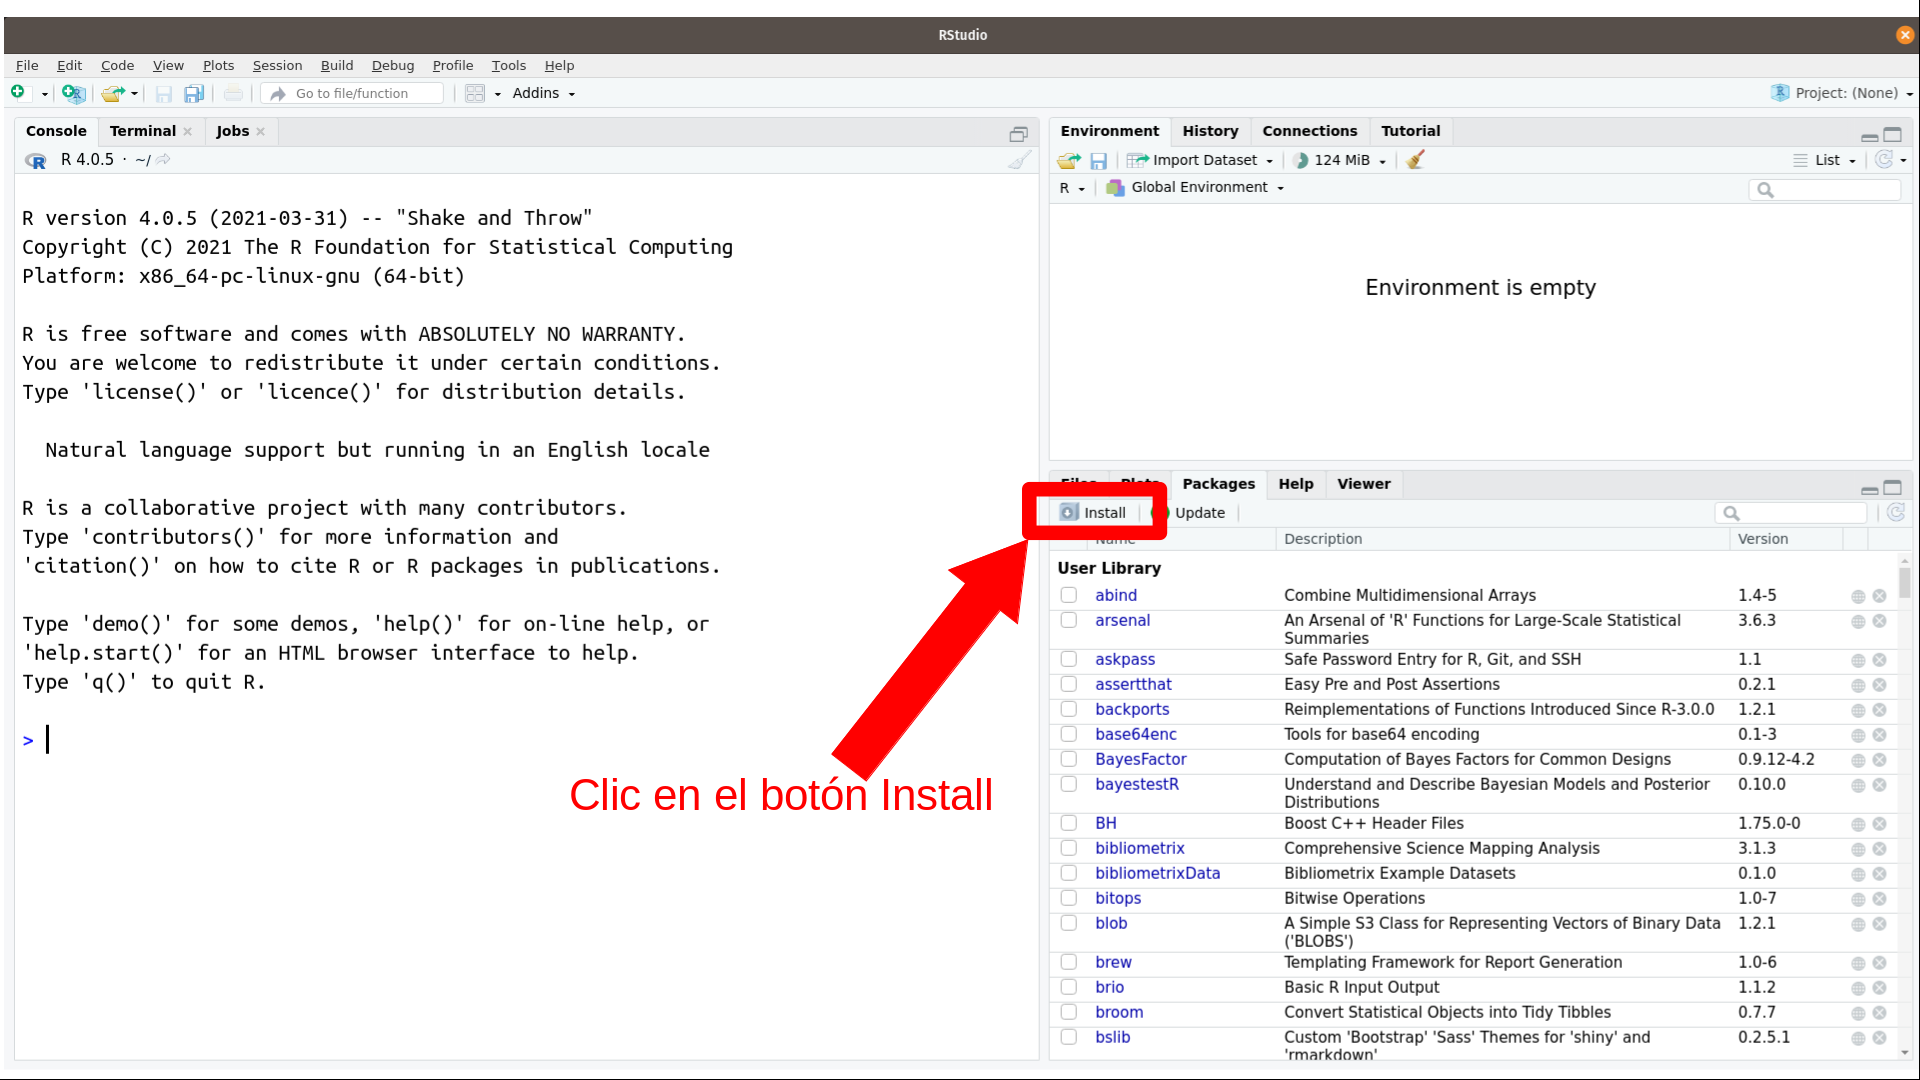
\includegraphics[width=.92\textwidth]{Paso2.png}
\end{figure}  
\end{frame}

\begin{frame}{ShinyItemAnalysis: Paso 4}
\begin{figure}
\centering
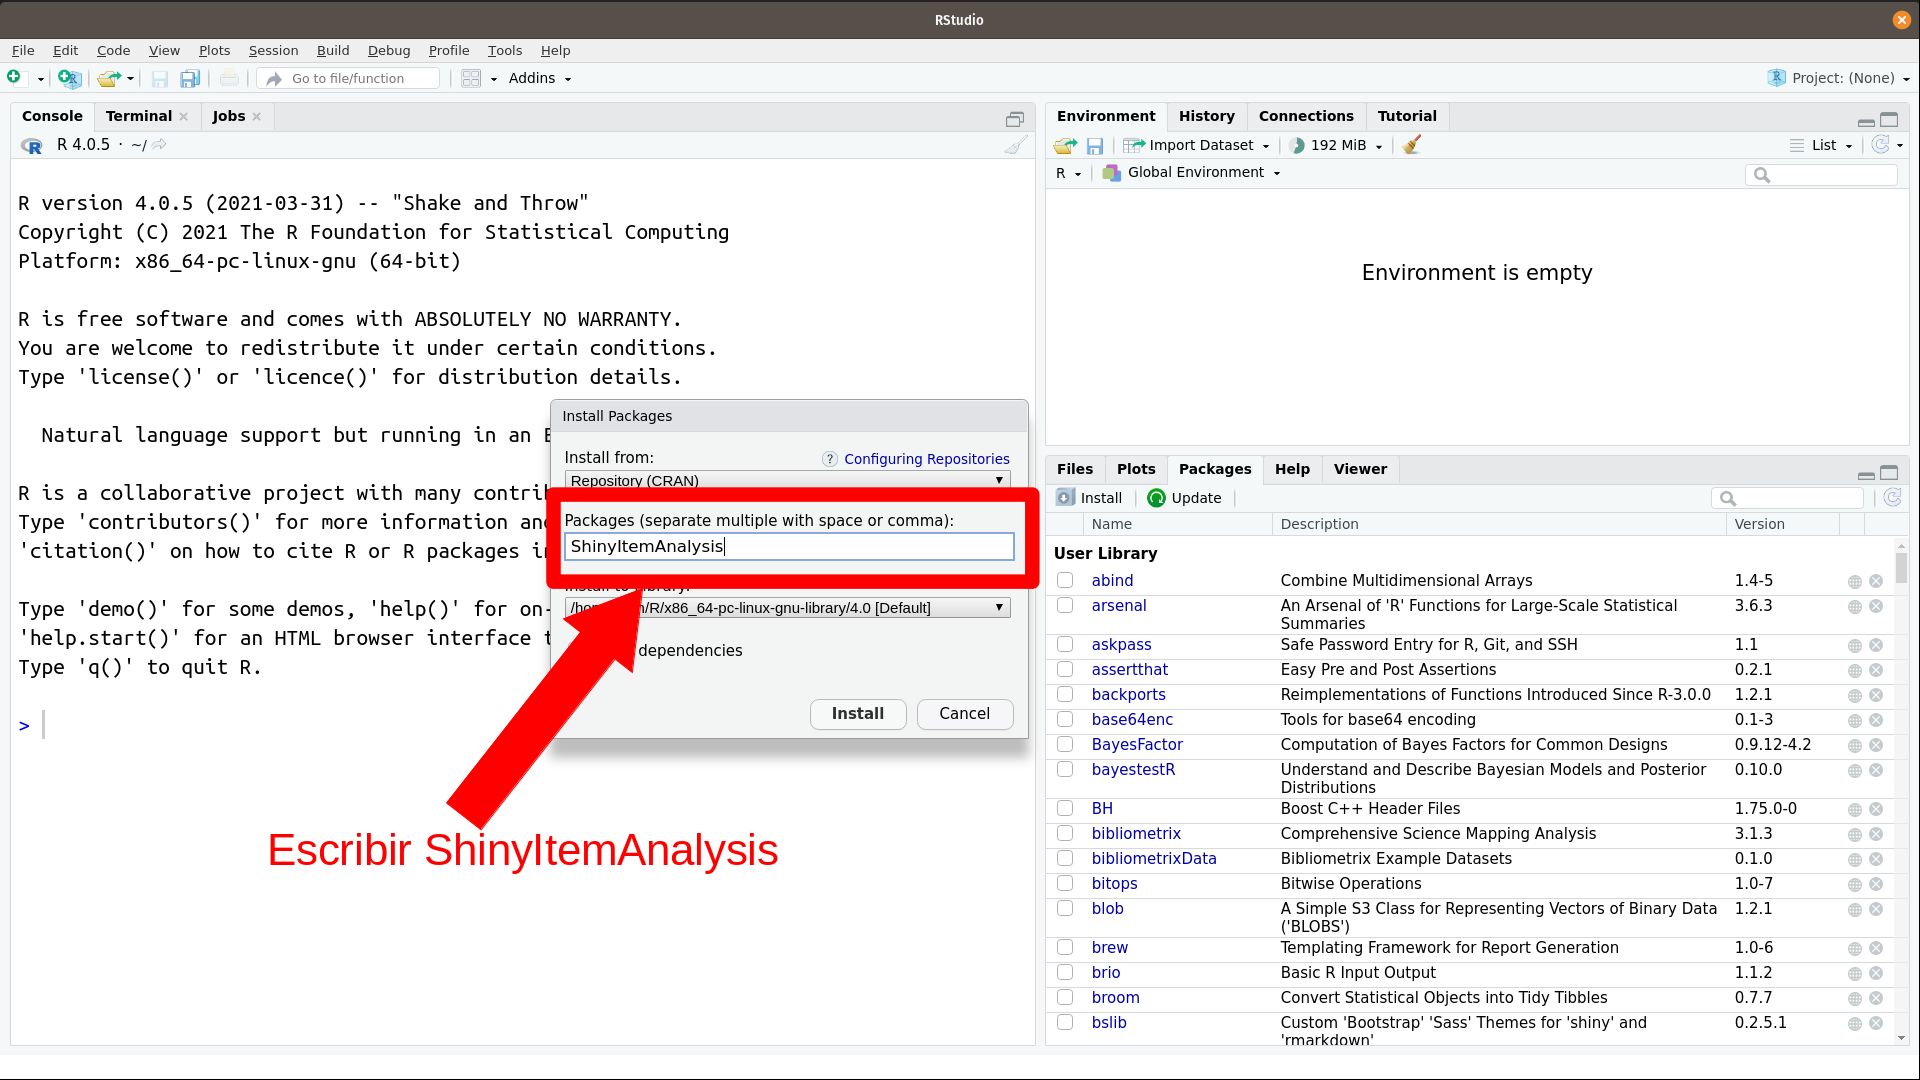
\includegraphics[width=.92\textwidth]{Paso3.png}
\end{figure}  
\end{frame}

\begin{frame}{ShinyItemAnalysis: Paso 5}
\begin{figure}
\centering
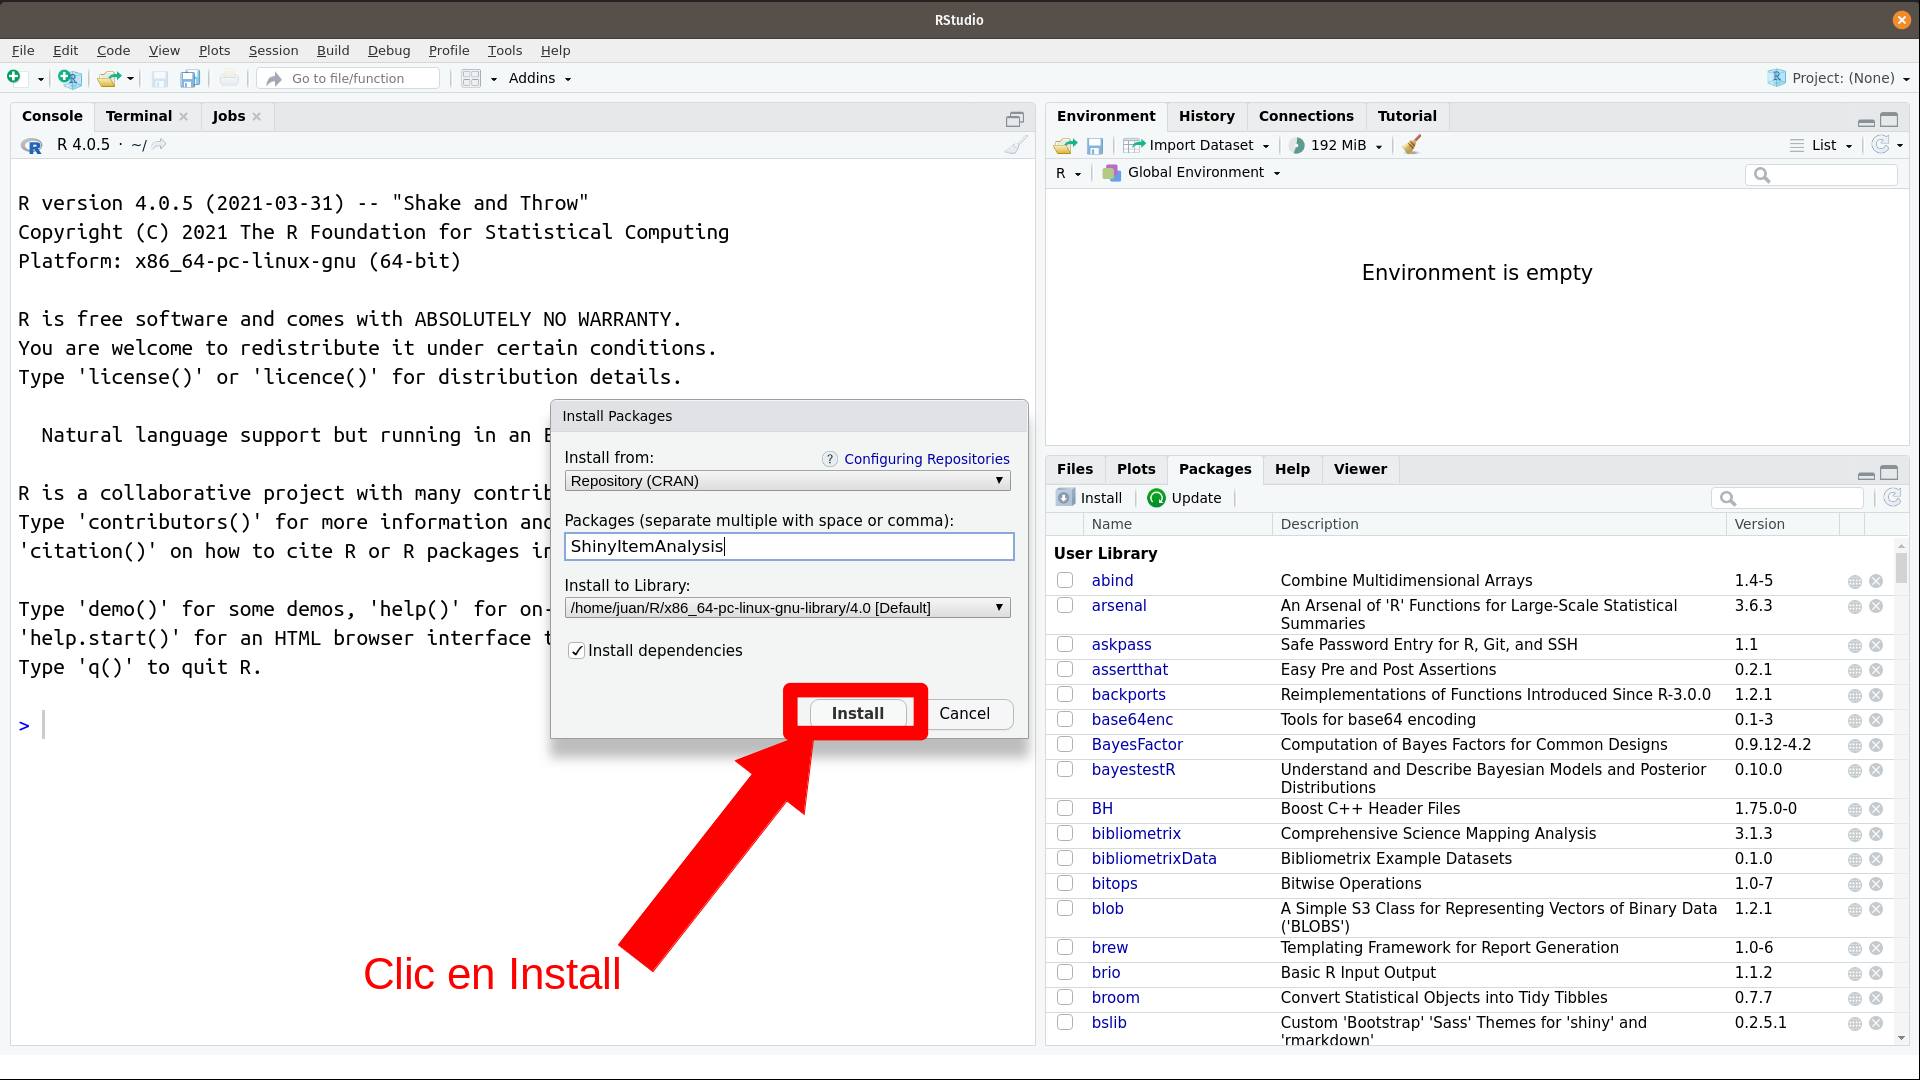
\includegraphics[width=.92\textwidth]{Paso4.png}
\end{figure}  
\end{frame}

\begin{frame}{ShinyItemAnalysis: Paso 6}
Apariencia de la Console mientras se instala el paquete.
\begin{figure}
\centering
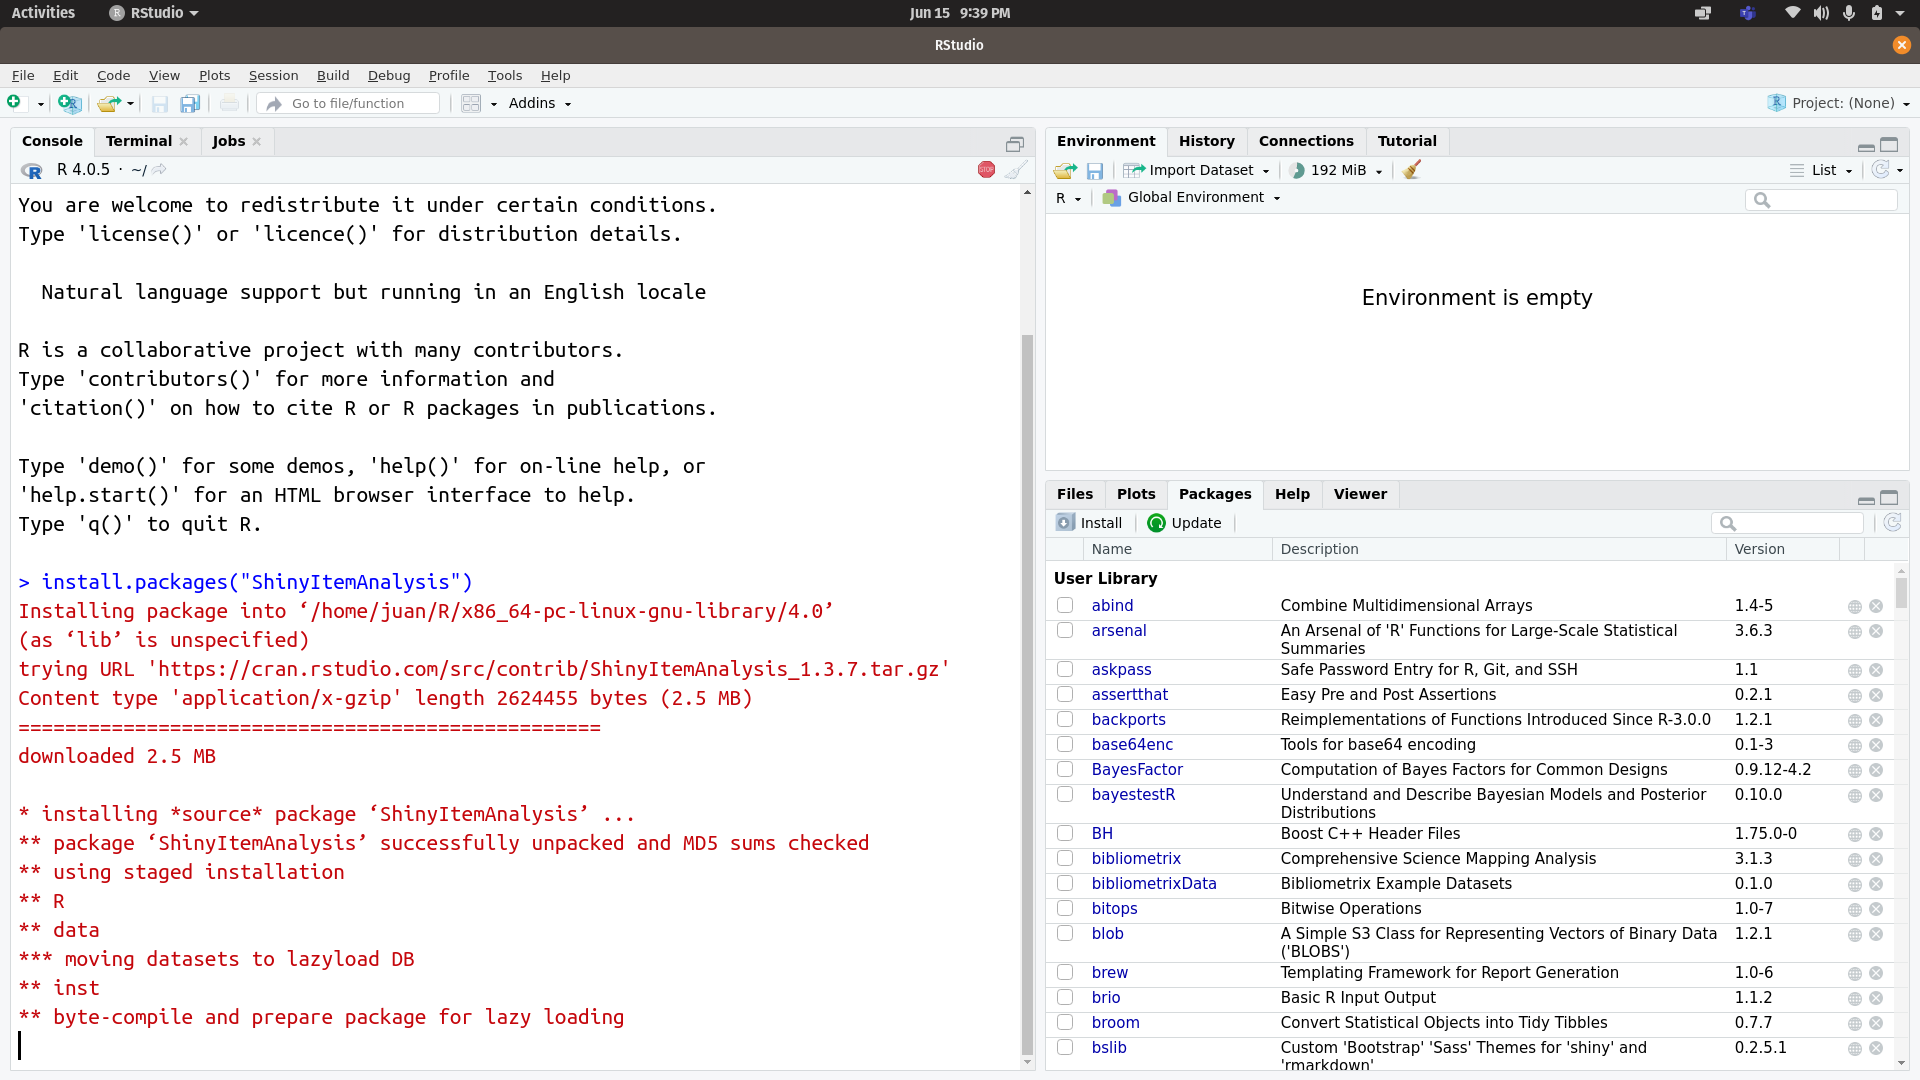
\includegraphics[width=.85\textwidth]{Paso5.png}
\end{figure}  
\end{frame}

\begin{frame}{ShinyItemAnalysis: Paso 7}
Apariencia de la Console en Rstudio luego de la instalación exitosa del paquete.
\begin{figure}
\centering
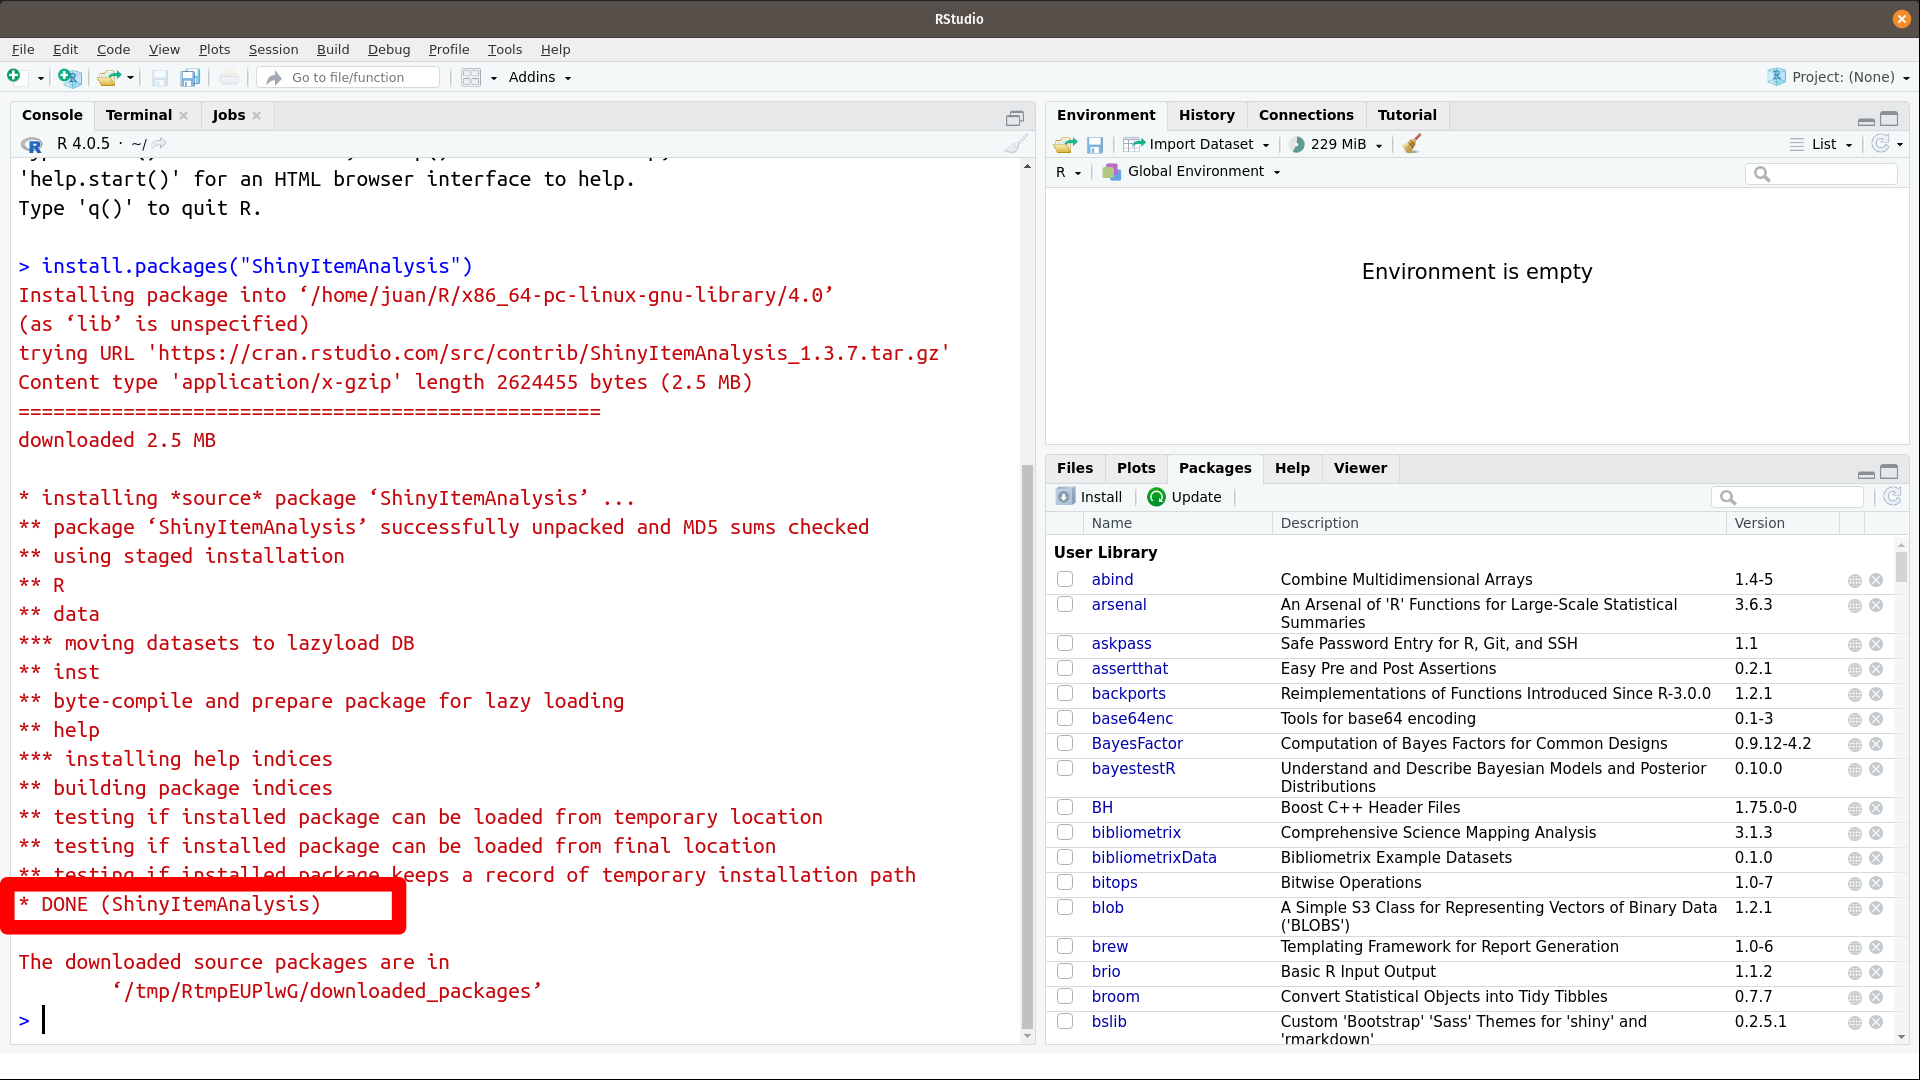
\includegraphics[width=.85\textwidth]{Paso6.png}
\end{figure}  
Verifique la presencia del siguiente mensaje en la Console\\
\textcolor{red}{\texttt{* DONE (ShinyItemAnalysis)}}
\end{frame}

\begin{frame}{ShinyItemAnalysis: Paso 8}
Ingresemos a la herramienta ShinyItemAnalysis
\begin{figure}
\centering
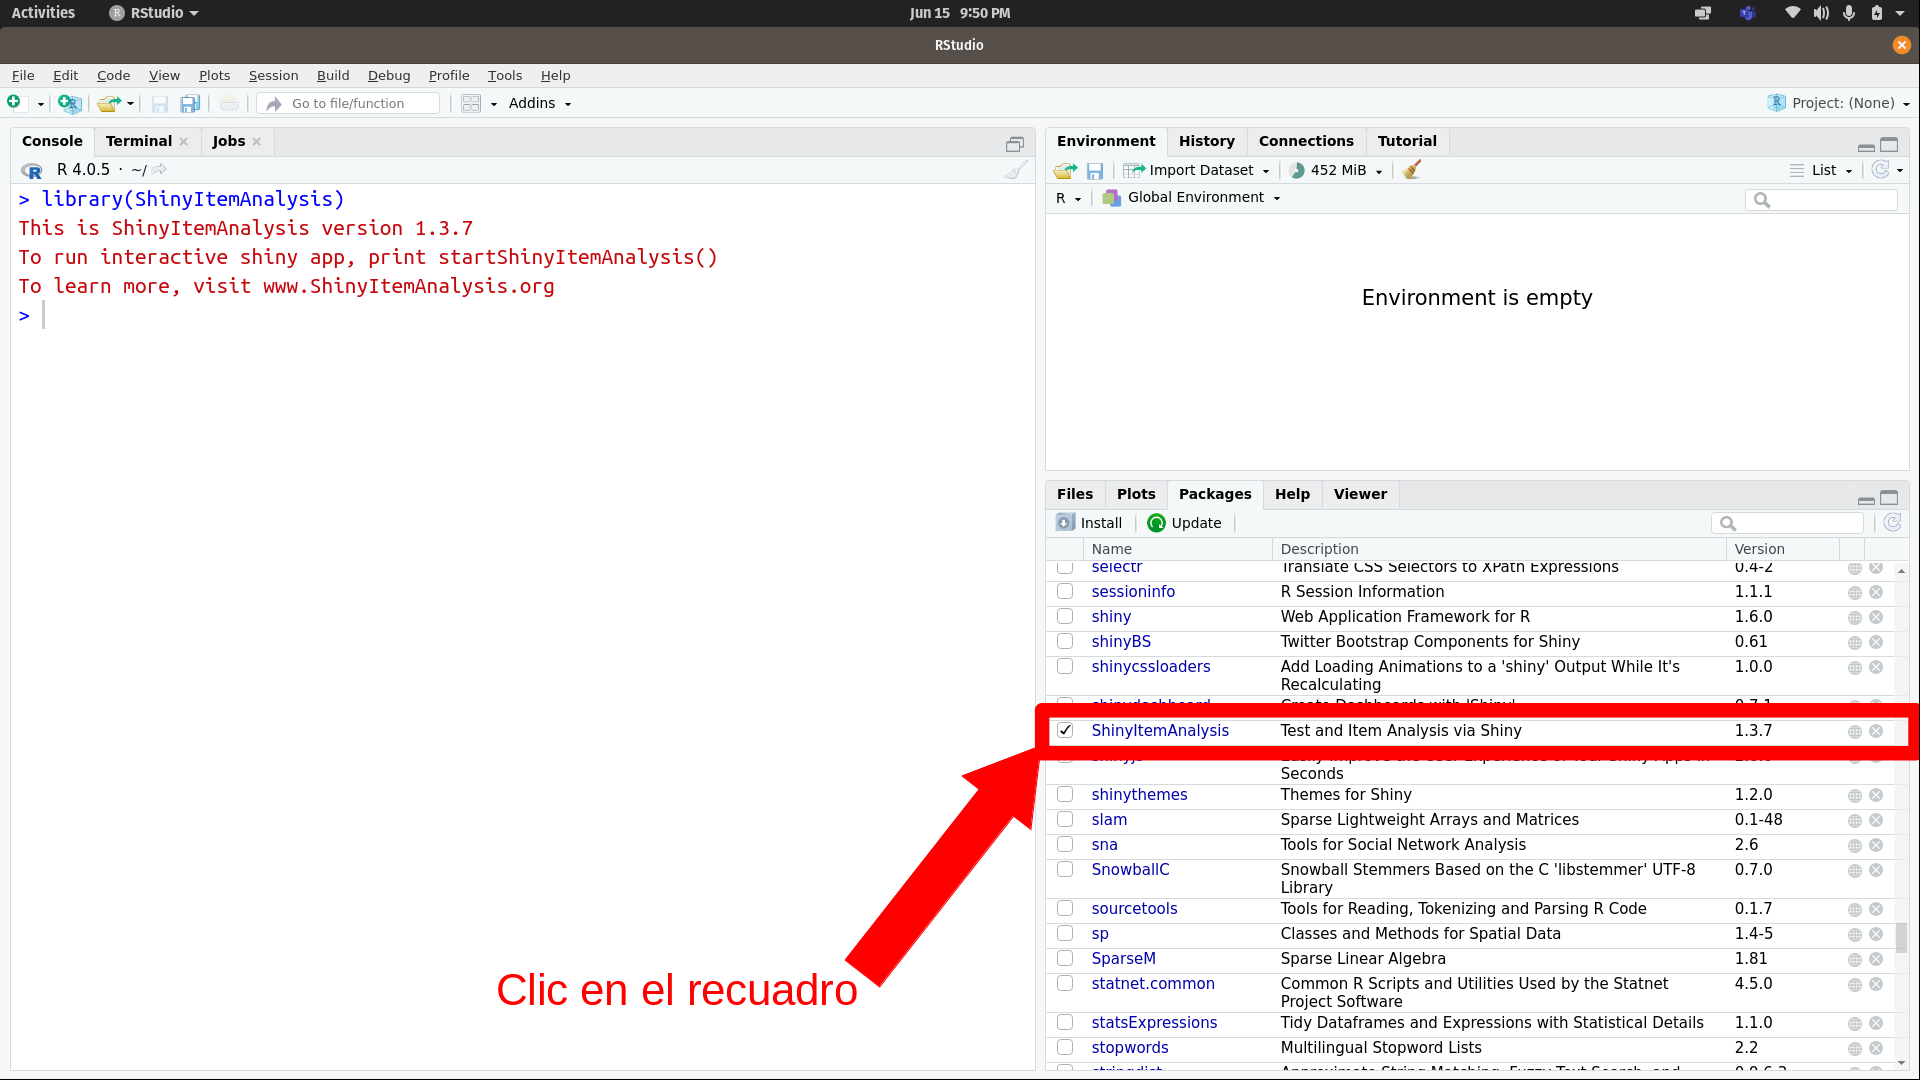
\includegraphics[width=.85\textwidth]{Paso7.png}
\end{figure}  
\end{frame}


\begin{frame}{ShinyItemAnalysis: Paso 9}
Vamos a ingresar a la herramienta  \texttt{ShinyItemAnalysis} escribiendo el código \texttt{startShinyItemAnalysis}
\begin{figure}
\centering
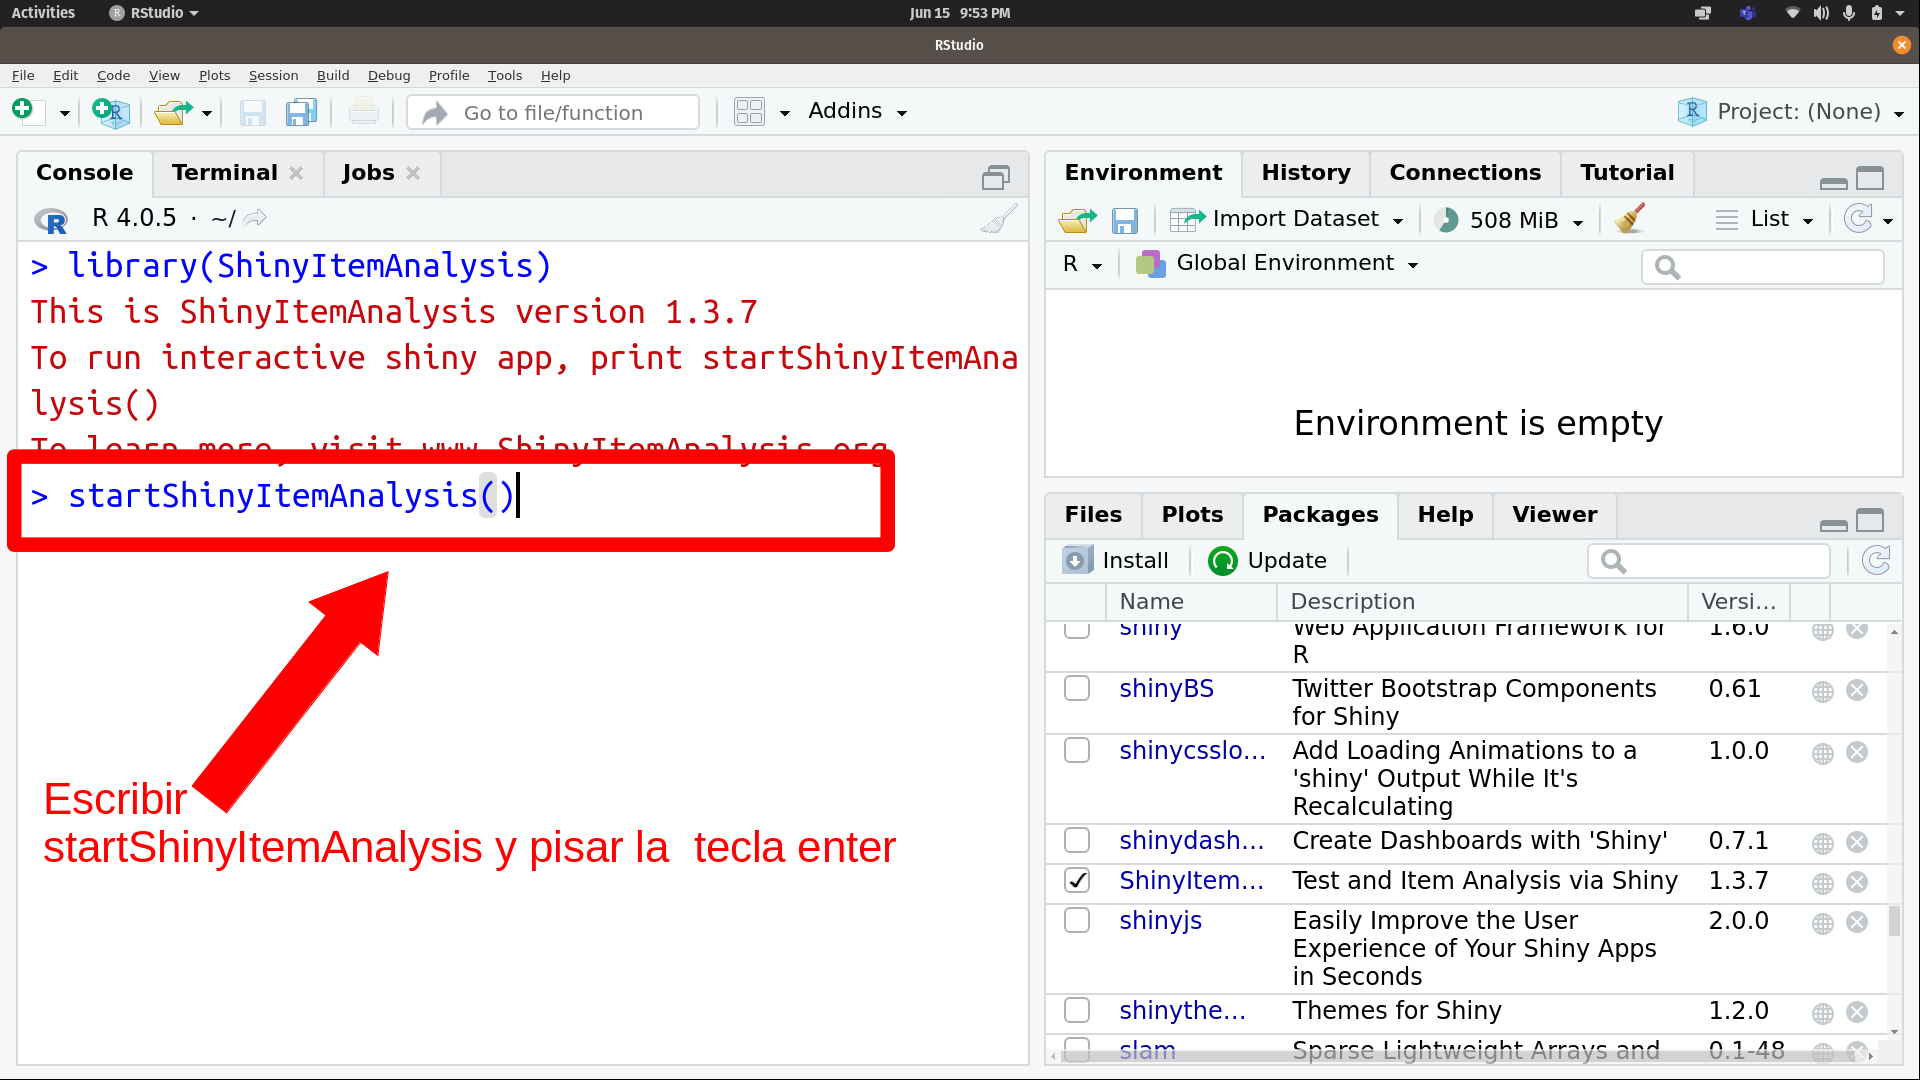
\includegraphics[width=.85\textwidth]{Paso8.png}
\end{figure}  
\end{frame}

\begin{frame}{ShinyItemAnalysis: Paso 10}
Apariencia de la herramienta ShinyItemAnalysis dentro de su navegador de Internet
\begin{figure}
\centering
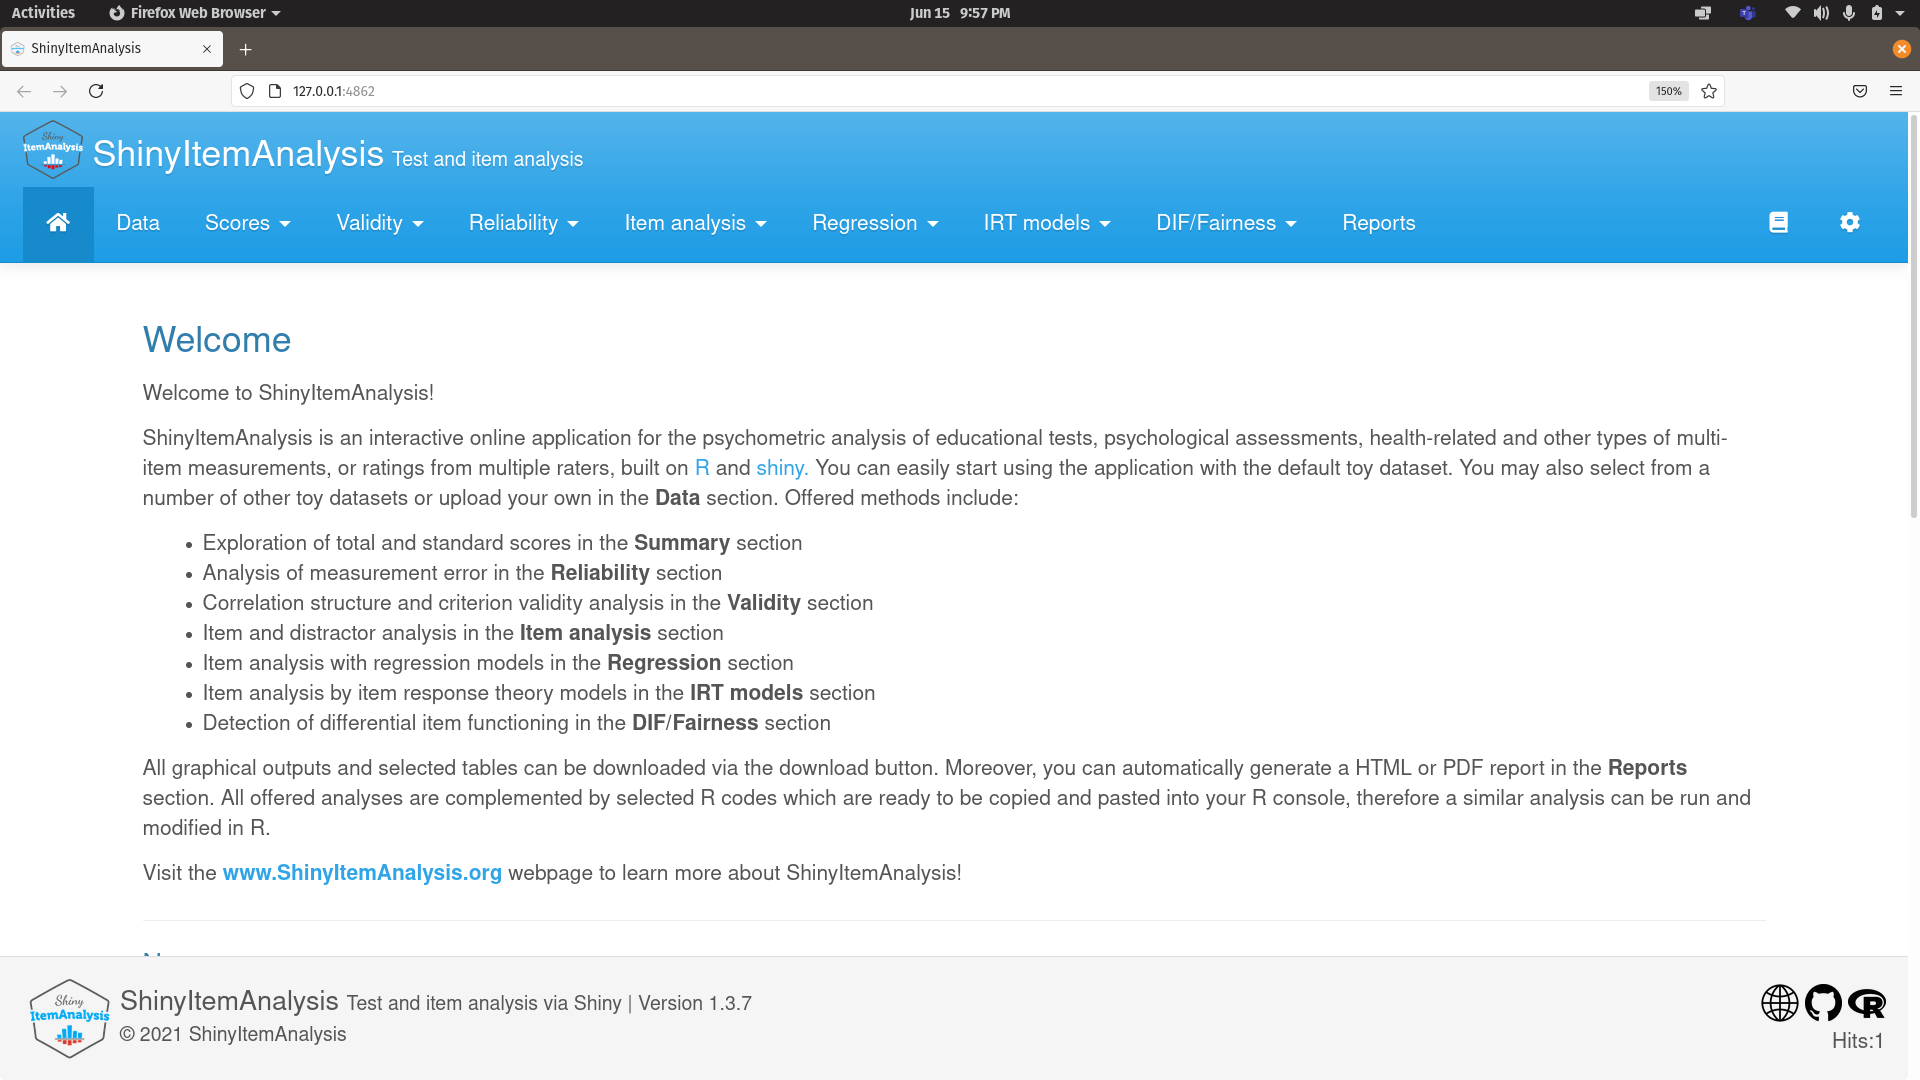
\includegraphics[width=.85\textwidth]{Paso9.png}
\end{figure}  
\end{frame}

\begin{frame}{ShinyItemAnalysis: Paso 11}
Seleccione los datos disponibles y explore las opciones disponibles en los menues ``Validity'', ``Reliability'', ``Item Analysis'', ``Regression'', ``IRT Models'', ``DIF/Fairness'' y ``Reports''.
\begin{figure}
\centering
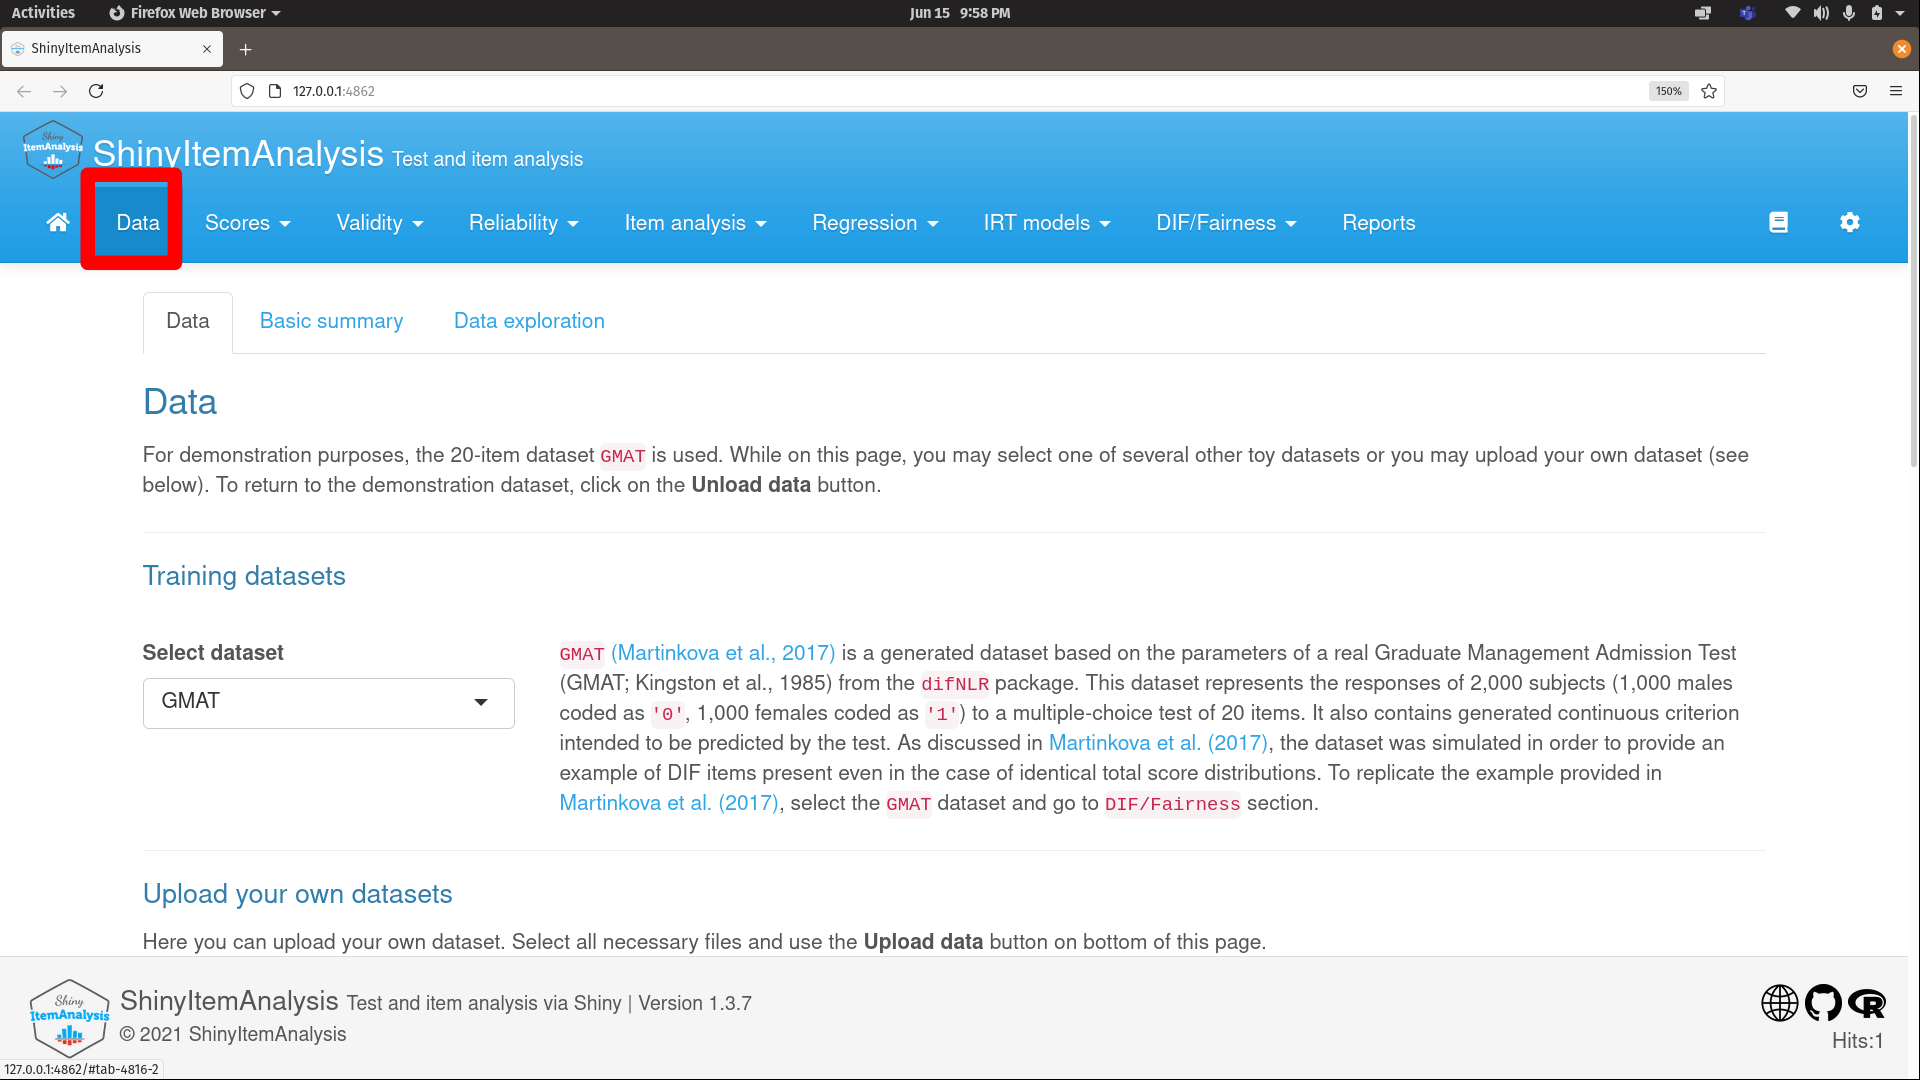
\includegraphics[width=.85\textwidth]{Paso10.png}
\end{figure}  
\end{frame}






\begin{frame}[allowframebreaks]{Referencias}
\tiny{ 
\bibliographystyle{apacite}
\bibliography{refs}
}
\end{frame}


\end{document}